Pac-Man is a maze-chase video game developed in 1980s. 
The player controls the character ``Pac-Man'' to eat dots in a maze while
avoiding enemy characters ``ghosts.'' 
All characters may move in four directions: up, down, left, right.
The game ends in two conditions:
\begin{itemize}
\tightlist
\item Pac-Man eats all dots in the maze. In this case, the player wins.
\item Any ghost catches Pac-Man. In this case, the player loses.
\end{itemize}

\begin{figure}[h]
\center
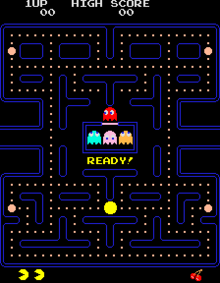
\includegraphics[width=0.25\textwidth]{image/pacman.png}
\caption{Pac-Man gameplay (image from Wikipedia)}
\end{figure}

Adam is learning how to create games with modern programming tools.
To practice the skills, he tries to make an imitation of the Pac-Man 
game with some modification.
In Adam's game, the playable character is a ``ghost,'' 
and the enemy character is ``Pac-Man.'' 
Since he changes the roles of the ghost and Pac-Man, 
he also changes the ending conditions of the game.
\begin{itemize}
\tightlist
\item Pac-Man eats all dots in the maze. In this case, the player loses.
\item The ghost controlled by the player catches Pac-Man. In this case, the player wins.
\end{itemize}

Adam has almost developed the first full functioning version of his game.
He wants to test his game and creates a simple stage for testing.
The maze of the stage is based on 10-by-10 grid. 
We label the cell lying at the intersection of row $r$ and column $c$ with 
$(r,c)$.
Each grid cell contains exact one dot.
The exterior boundary of the grid are walls. 
No characters may move to the area outside of the grid.
Inside the grid, there are no walls or obstacles.
All characters may move freely from a cell to any cell adjacent to it.
Note that two grid cells $(r_1,c_1)$ and $(r_2,c_2)$ are adjacent to each other 
if and only if $|r_1-r_2|+|c_1+c_2|=1$.
 
Adam has to prepare the movements of Pac-Man for the testing. 
He need a set of trajectory with diversity, 
but any of the trajectory must satisfy the following requirements.
\begin{itemize}
\tightlist
\item Pac-Man can eat all dots in the maze if it follows the trajectory.
\item Pac-Man moves at most 10000 steps.
\end{itemize}
Adam need your help to generate a trajectory starting at cell $(x,y)$.
Please write a program to generate a trajectory of Pac-Man satisfying all 
requirements above and starting at cell $(x,y)$.

